\documentclass{beamer}
 
\usepackage[utf8]{inputenc}
 
\usetheme{Madrid} 

\usepackage{natbib}
\bibliographystyle{chicago}

\begin{document}

\title[Parameter estimation] %optional
{Estimating time-varying transmission rates of the SIR model}

\author[Sang Woo Park] % (optional, for multiple authors)
{Sang Woo Park}

\institute[McMaster University] % (optional)
{
    Department of Mathematics and Statistics\\
    McMaster University
}

\date[2019] % (optional)
{April 10, 2019}

\frame{\titlepage}

\begin{frame}
\frametitle{Epidemic time series}
\begin{itemize}
    \item Measles report from the prevaccination era
\end{itemize}
\begin{center}
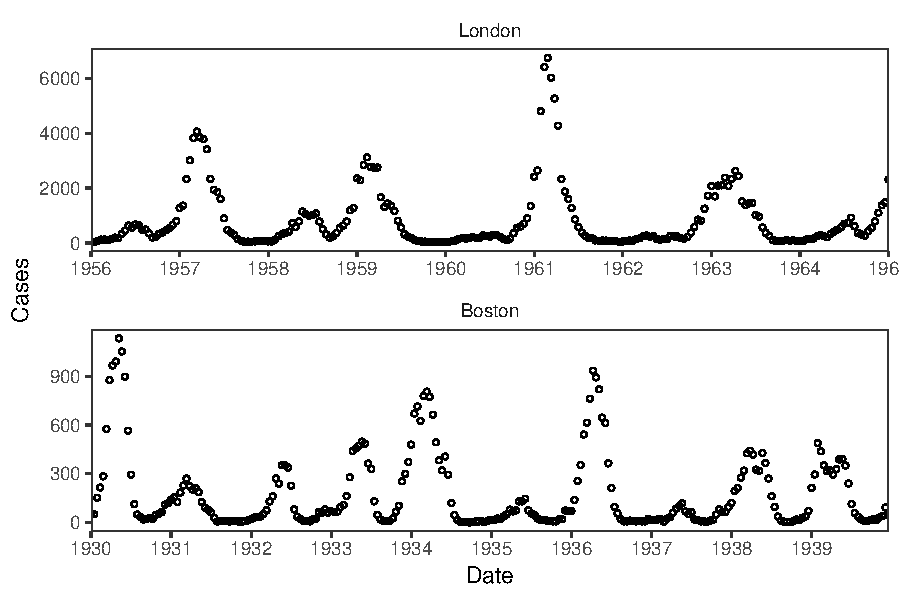
\includegraphics[width=0.9\textwidth]{fig1.pdf}
\end{center}
\end{frame}

\begin{frame}
\frametitle{Susceptible-Infected-Recovered (SIR) model}
\begin{itemize}
    \item Describes how disease spreads in a population
    \item Individuals move through compartments (Susceptible-Infected-Recovered)
\end{itemize}
\begin{center}
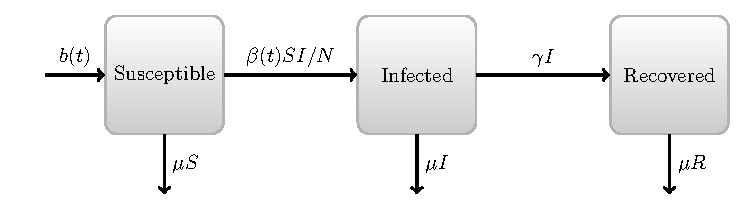
\includegraphics[width=\textwidth]{model_diagram.pdf}
\end{center}
\end{frame}

\begin{frame}
\frametitle{Susceptible-Infected-Recovered (SIR) model}
$$
\begin{aligned}
\frac{dS}{dt} &= b(t) - \beta(t) S \frac{I}{N} - \mu S\\
\frac{dI}{dt} &= \beta(t) S \frac{I}{N} - (\gamma + \mu) I\\
\frac{dR}{dt} &= \gamma I - \mu R
\end{aligned}
$$
\begin{itemize}
	\item Mean infectious period $1/\gamma$
	\item Mean life expectancy $1/\mu$
	\item Birth rate $b(t)$
	\item Transmission rate $\beta(t)$
\end{itemize}
\end{frame}

\begin{frame}
\frametitle{Trajectory matching}
\begin{itemize}
	\item Try to match the solution of the ODE with the observed time series
\end{itemize}
\begin{center}
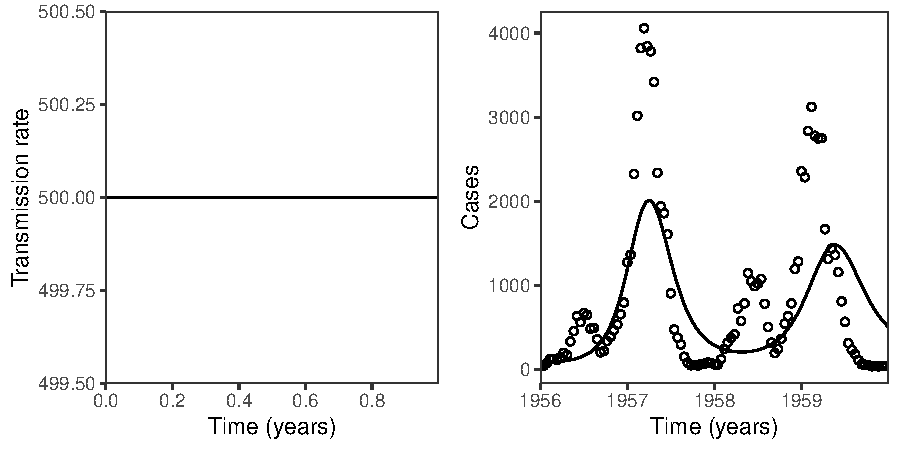
\includegraphics[width=\textwidth]{traj1.pdf}
\end{center}
\end{frame}

\begin{frame}
\frametitle{Trajectory matching}
\begin{itemize}
	\item Try to match the solution of the ODE with the observed time series
\end{itemize}
\begin{center}
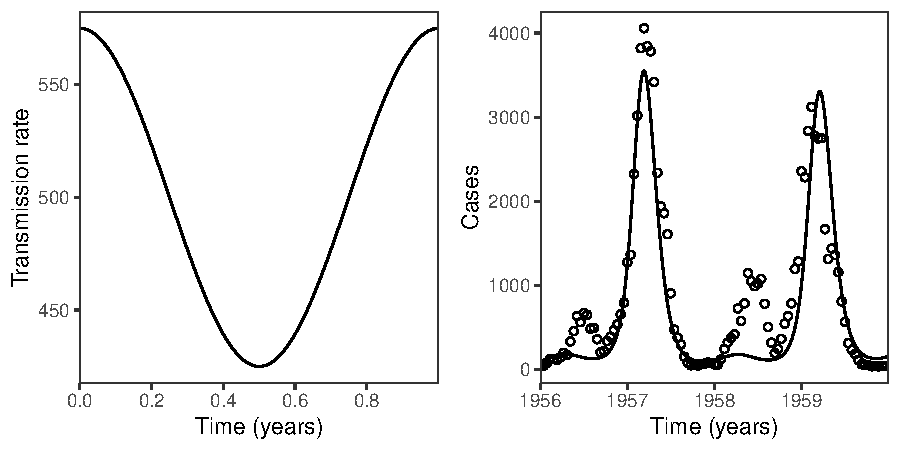
\includegraphics[width=\textwidth]{traj2.pdf}
\end{center}
\end{frame}

\begin{frame}
\frametitle{Trajectory matching}
\begin{itemize}
	\item Try to match the solution of the ODE with the observed time series
\end{itemize}
\begin{center}
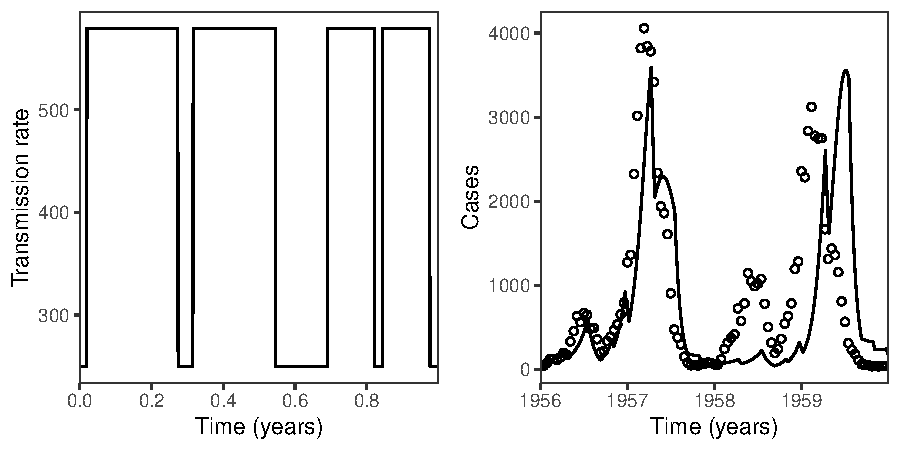
\includegraphics[width=\textwidth]{traj3.pdf}
\end{center}
\end{frame}

\begin{frame}
\frametitle{Gradient matching}
\begin{itemize}
	\item Try to match the gradient of the ODE with the estimated gradient
\end{itemize}
\begin{center}
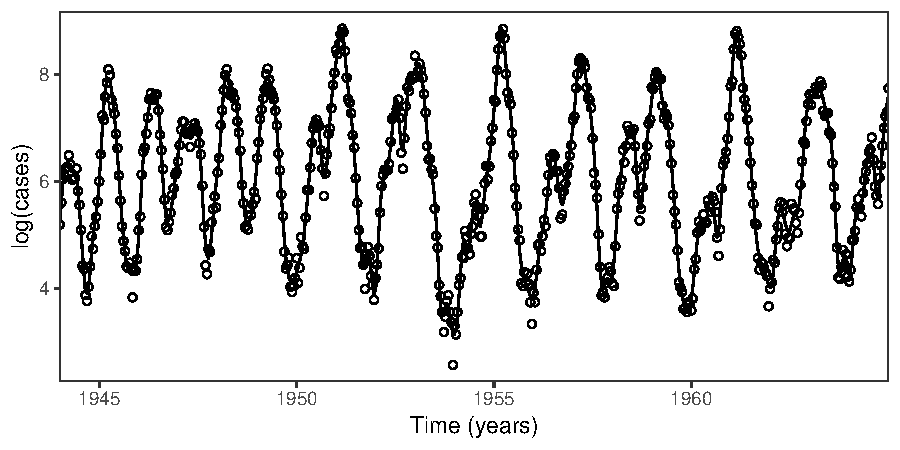
\includegraphics[width=\textwidth]{grad1.pdf}
\end{center}
\end{frame}

\begin{frame}
\frametitle{Gradient matching}
\begin{itemize}
	\item Estimate gradient by fitting a smooth curve and taking its derivative
\end{itemize}
\begin{center}
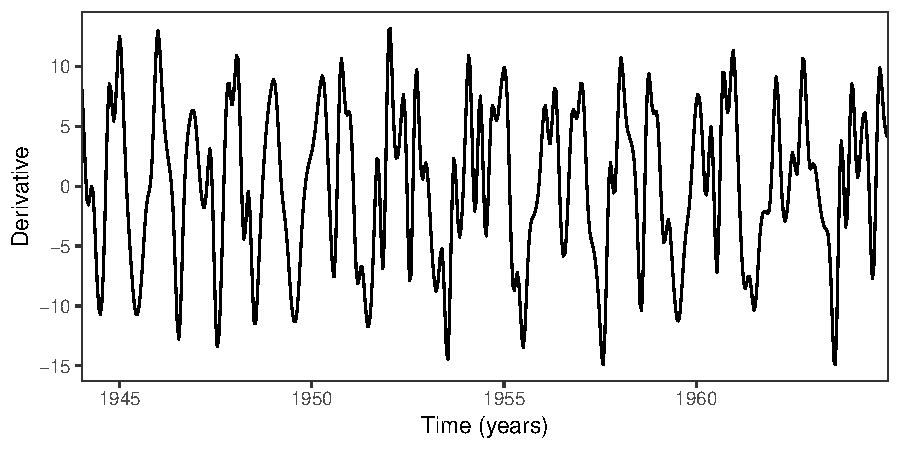
\includegraphics[width=\textwidth]{grad2.pdf}
\end{center}
\end{frame}

\begin{frame}
\frametitle{Gradient matching}
\begin{itemize}
	\item Match $d \log I/dt = \beta S - (\gamma + \mu)$ with the estimated derivative using a regression
	\item Reconstruct $S$ from birth and case reports
\end{itemize}
\begin{center}
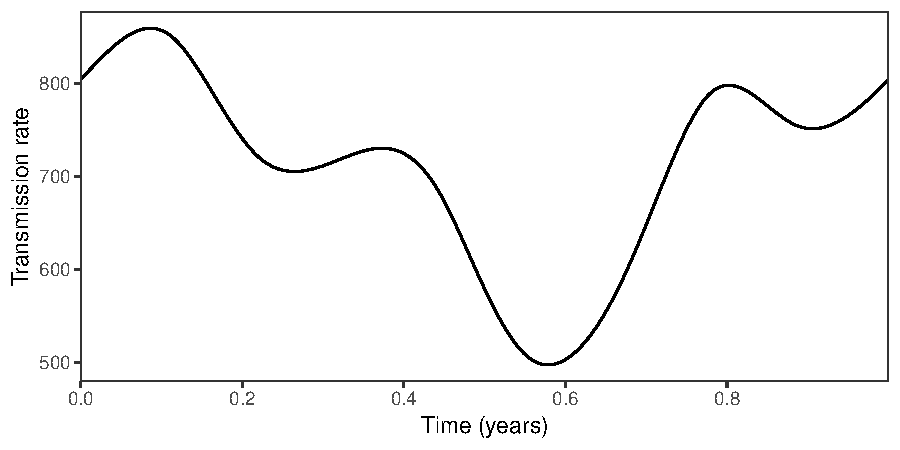
\includegraphics[width=\textwidth]{grad3.pdf}
\end{center}
\end{frame}







\begin{frame}
\frametitle{References}
\tiny
% \bibliography{plague}
\end{frame}

\end{document}
